\section{Mass fits for signal and normalization}
\label{sec: fitting}

This section describes the fits to the invariant mass distribution of $\Bs\to\Ds\kaon\pion\pion$ and $\Bs\to\Ds\pion\pion\pion$ candidates after all selections are applied. 
The obtained yields are summarized in Tab. \ref{tab: SigYields}.

\subsection{Fit to $\Bs\to\Ds\pion\pion\pion$ candidates}
\label{subsec: NormFit}

An unbinned maximum likelihood fit is performed simultaneously to the invariant mass distribution of $\Bs\to\Ds\pion\pion\pion$ candidates, for 7 and 8 TeV data. 
As discussed in Sec. \ref{subsec: signalmodel}, the fit is given as the sum of the double Gaussian signal model, the sum of three bifurcated Gaussian functions to model the partially reconstructed $\Bs\to\Ds^{*}\pion\pion\pion$ background and an Exponential function to account for combinatorial background. The invariant mass distribution and the fit is shown in Fig. \ref{fig: BsDs3piFit}.

\begin{figure}[h]
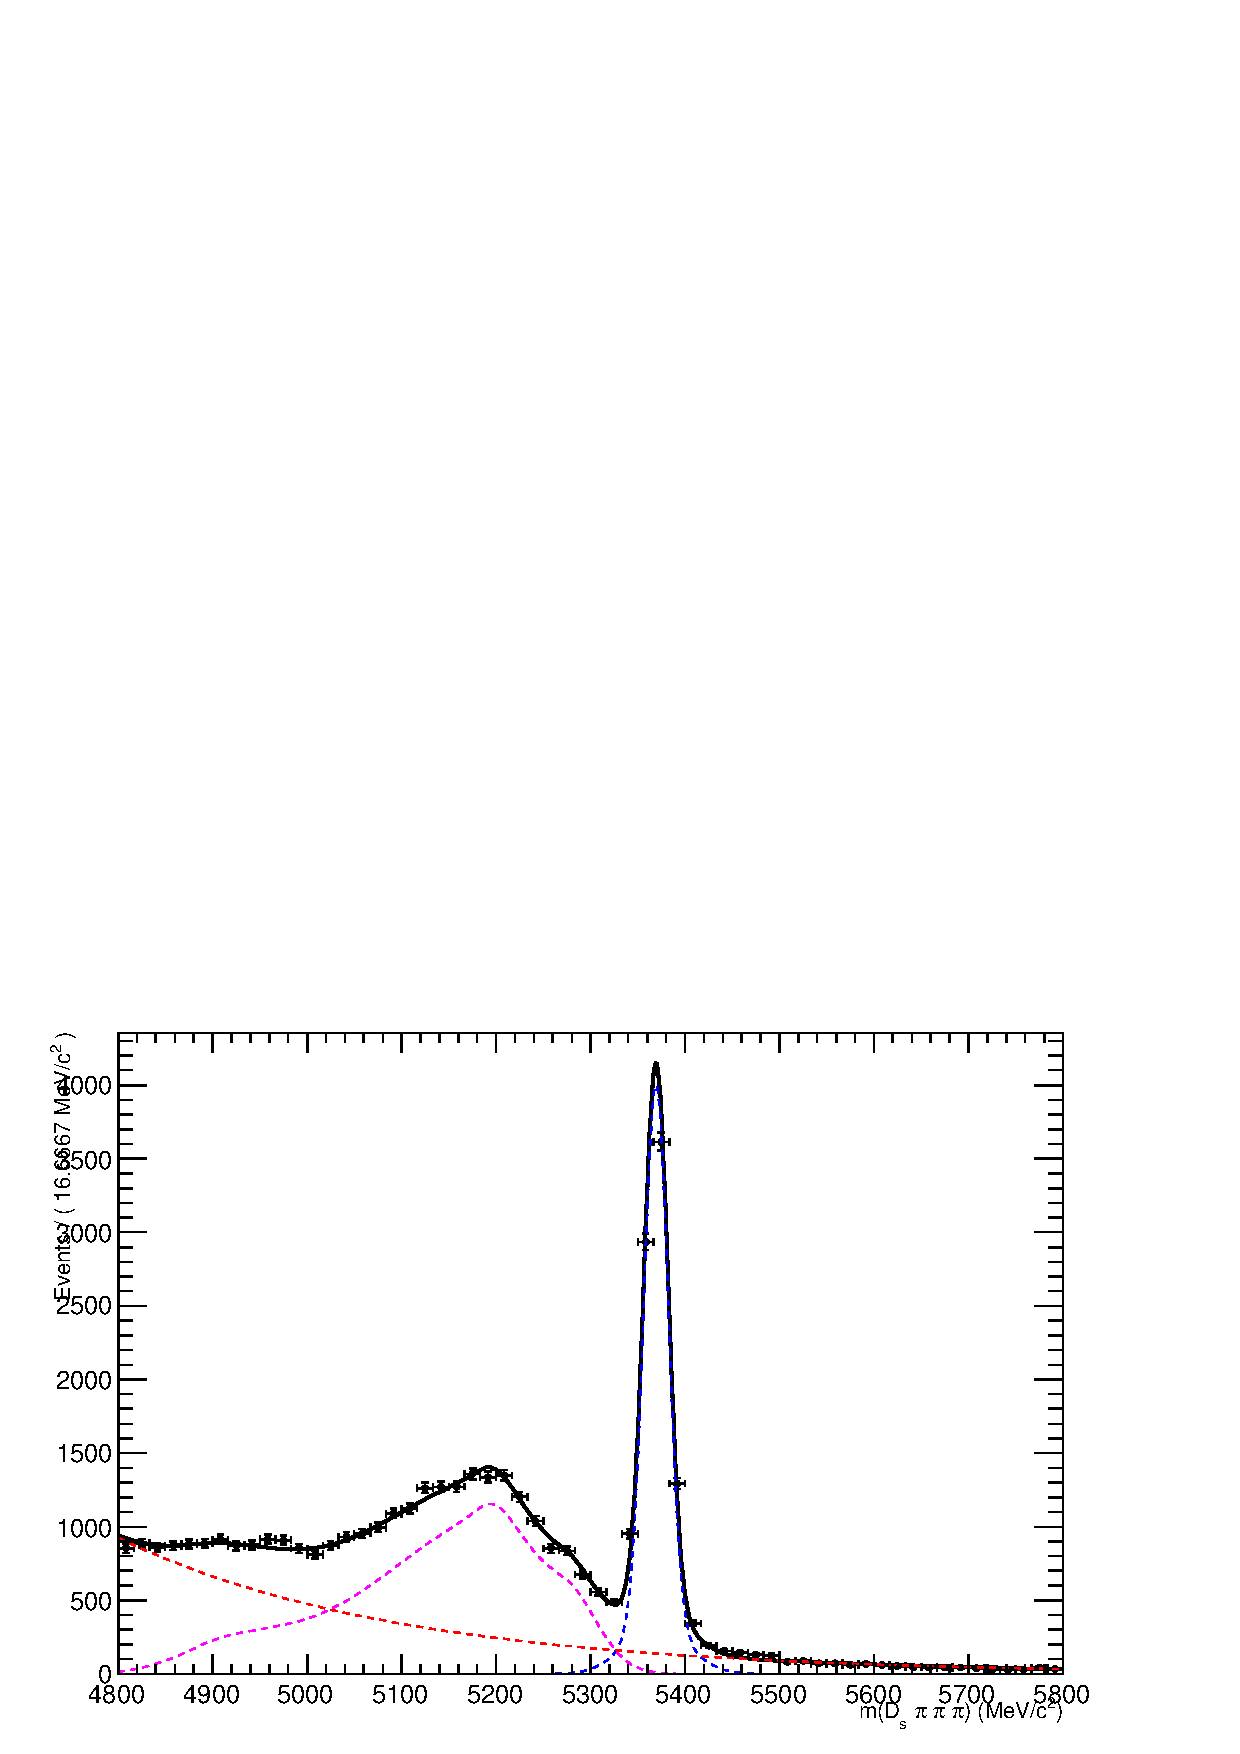
\includegraphics[height=7.cm,width=0.49\textwidth]{figs/3pi_BmassFit_sim11.pdf}
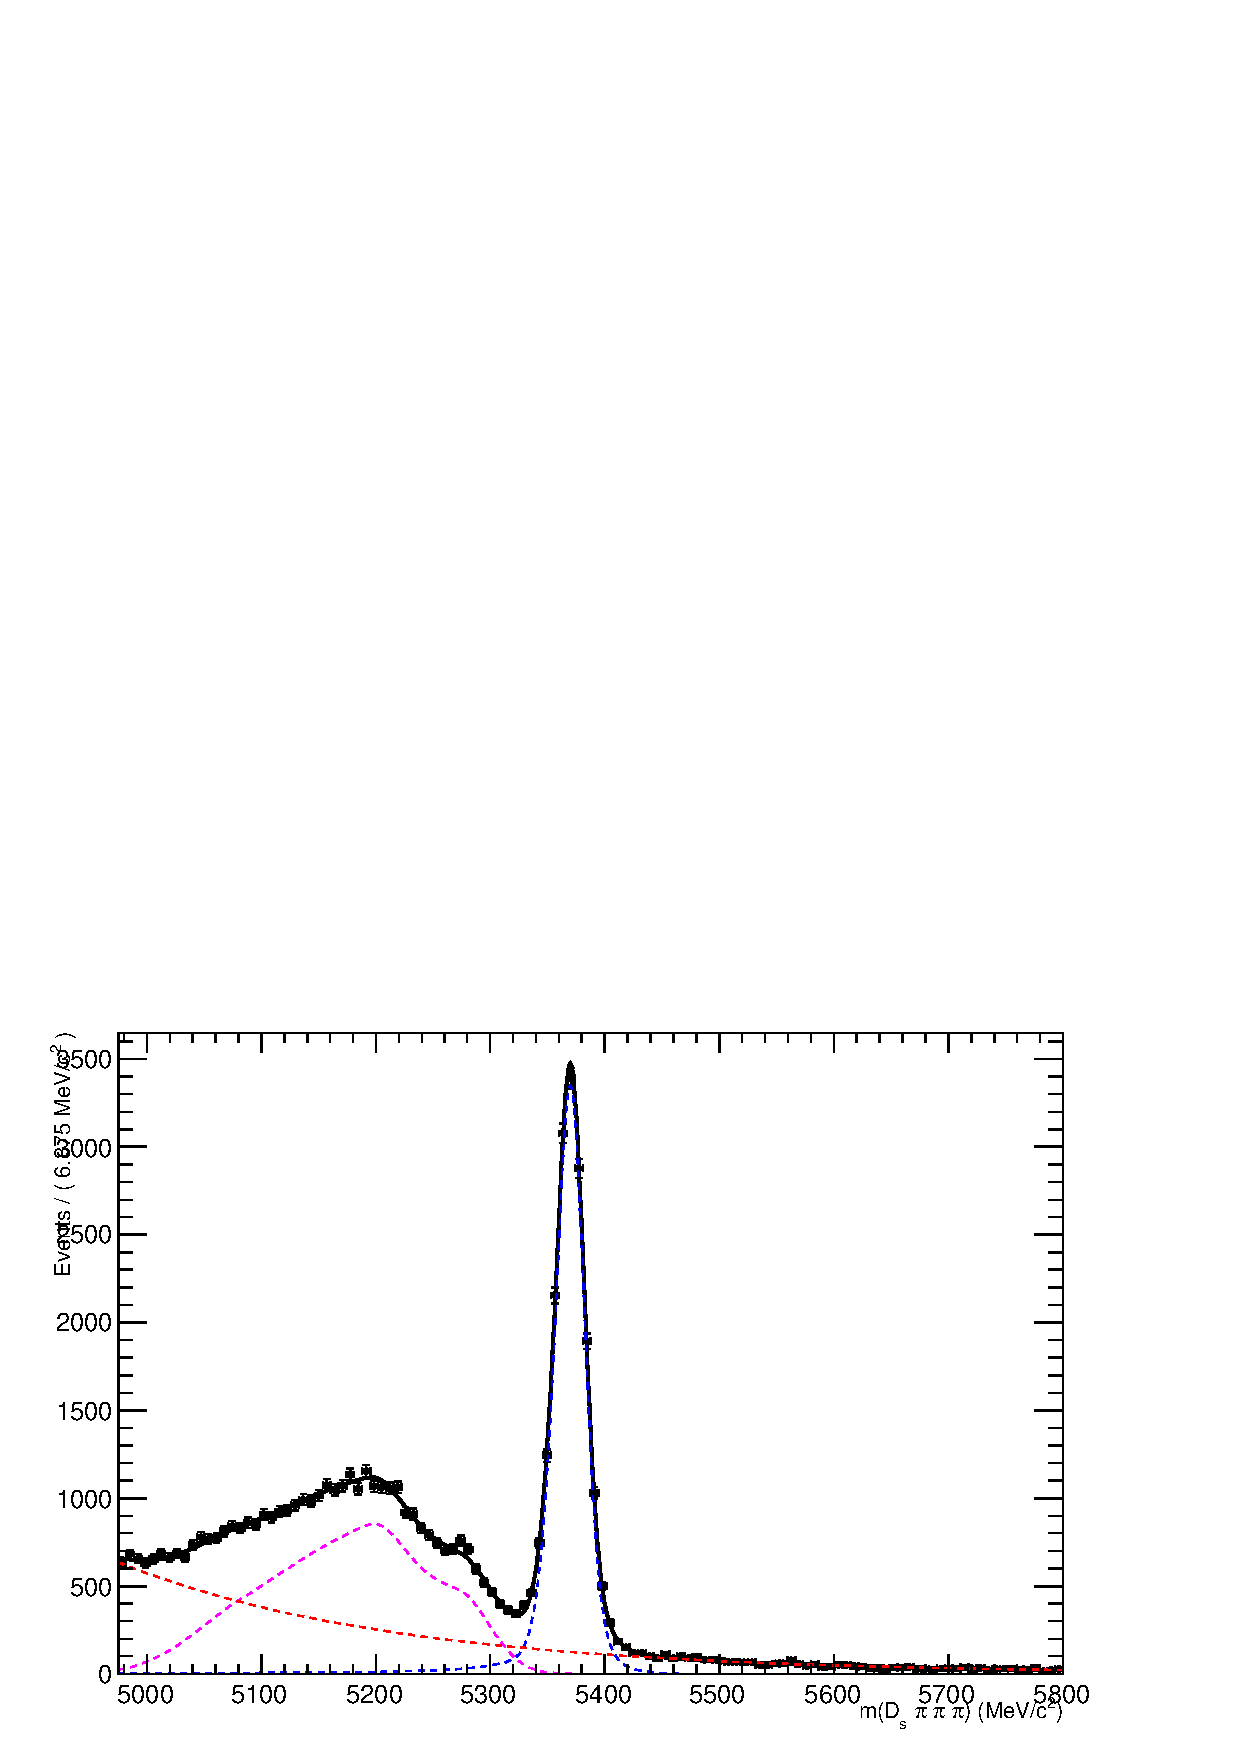
\includegraphics[height=7.cm,width=0.49\textwidth]{figs/3pi_BmassFit_sim12.pdf}\\
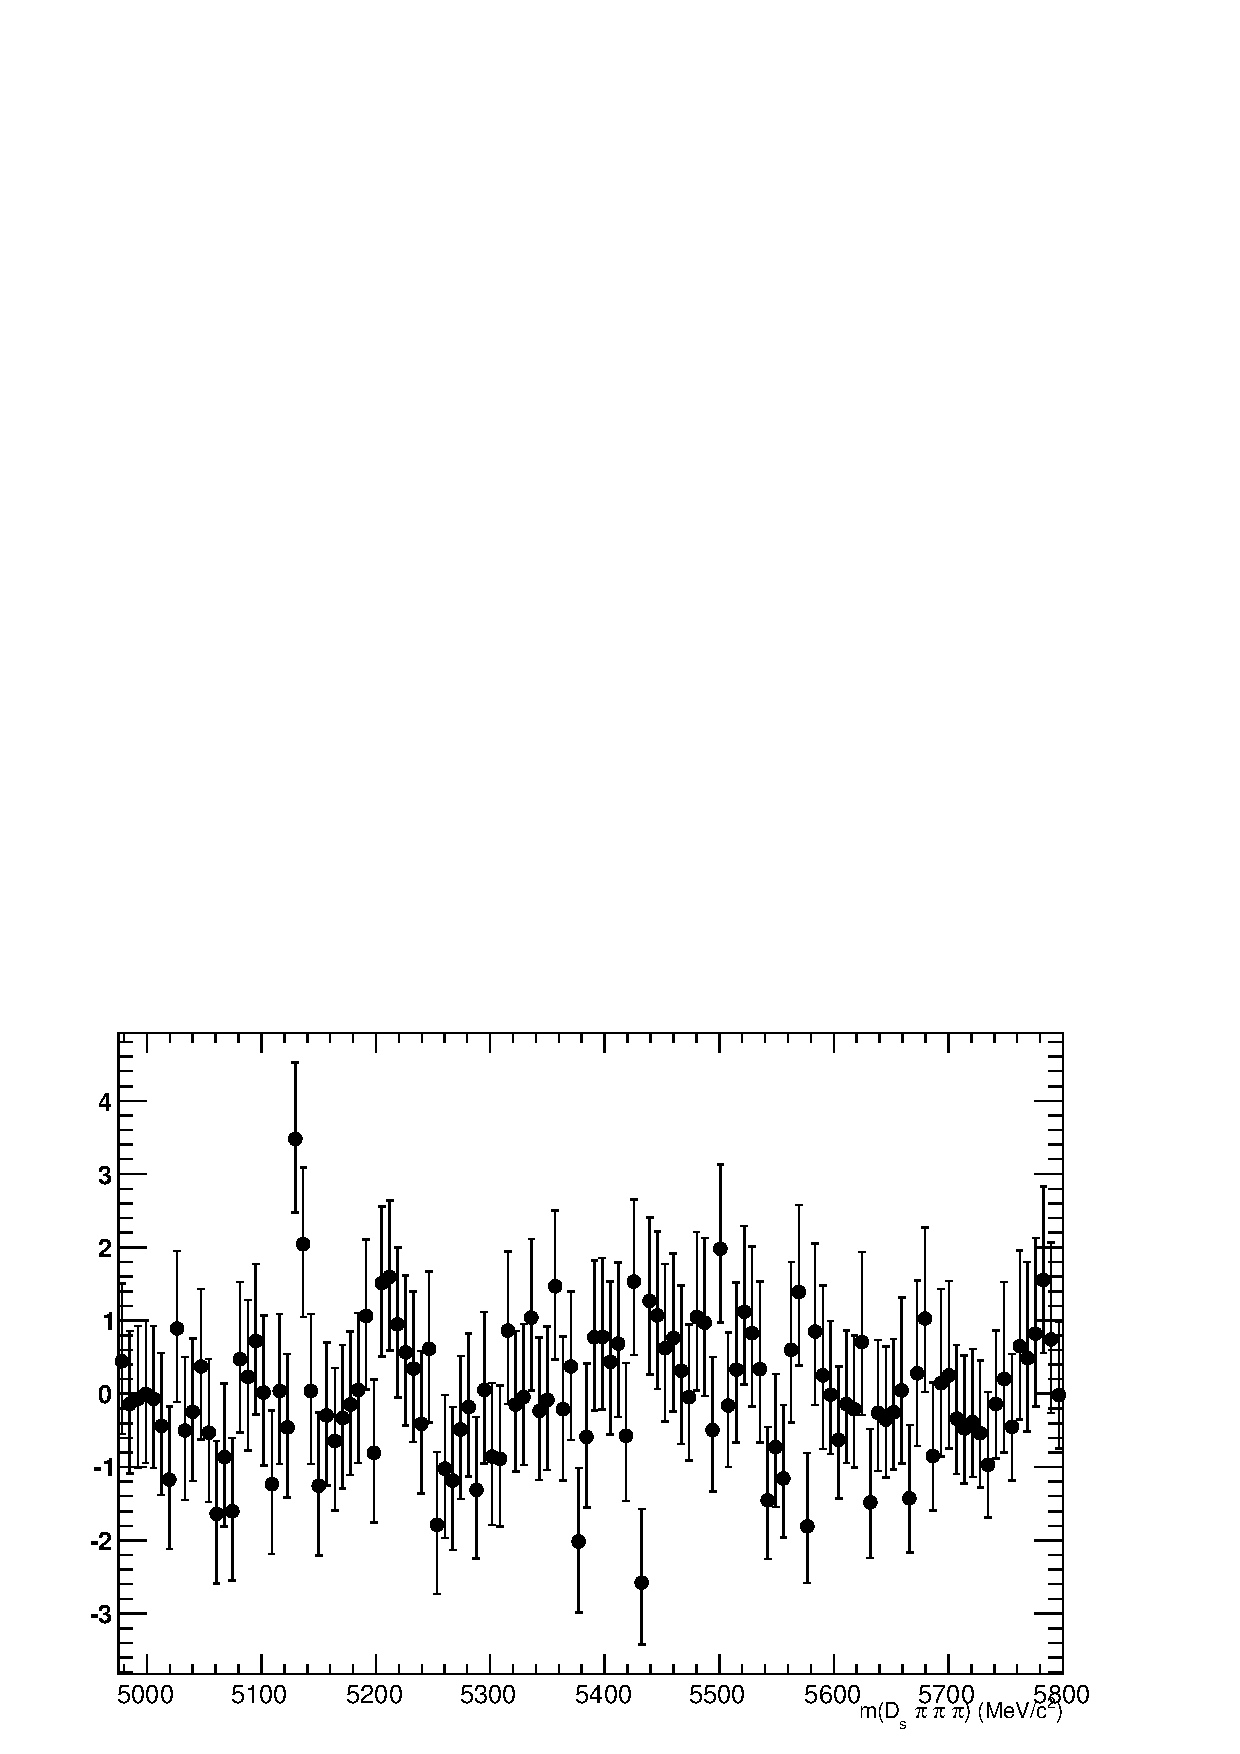
\includegraphics[width=0.49\textwidth,height=1.5cm]{figs/3pi_pull_sim11.pdf}
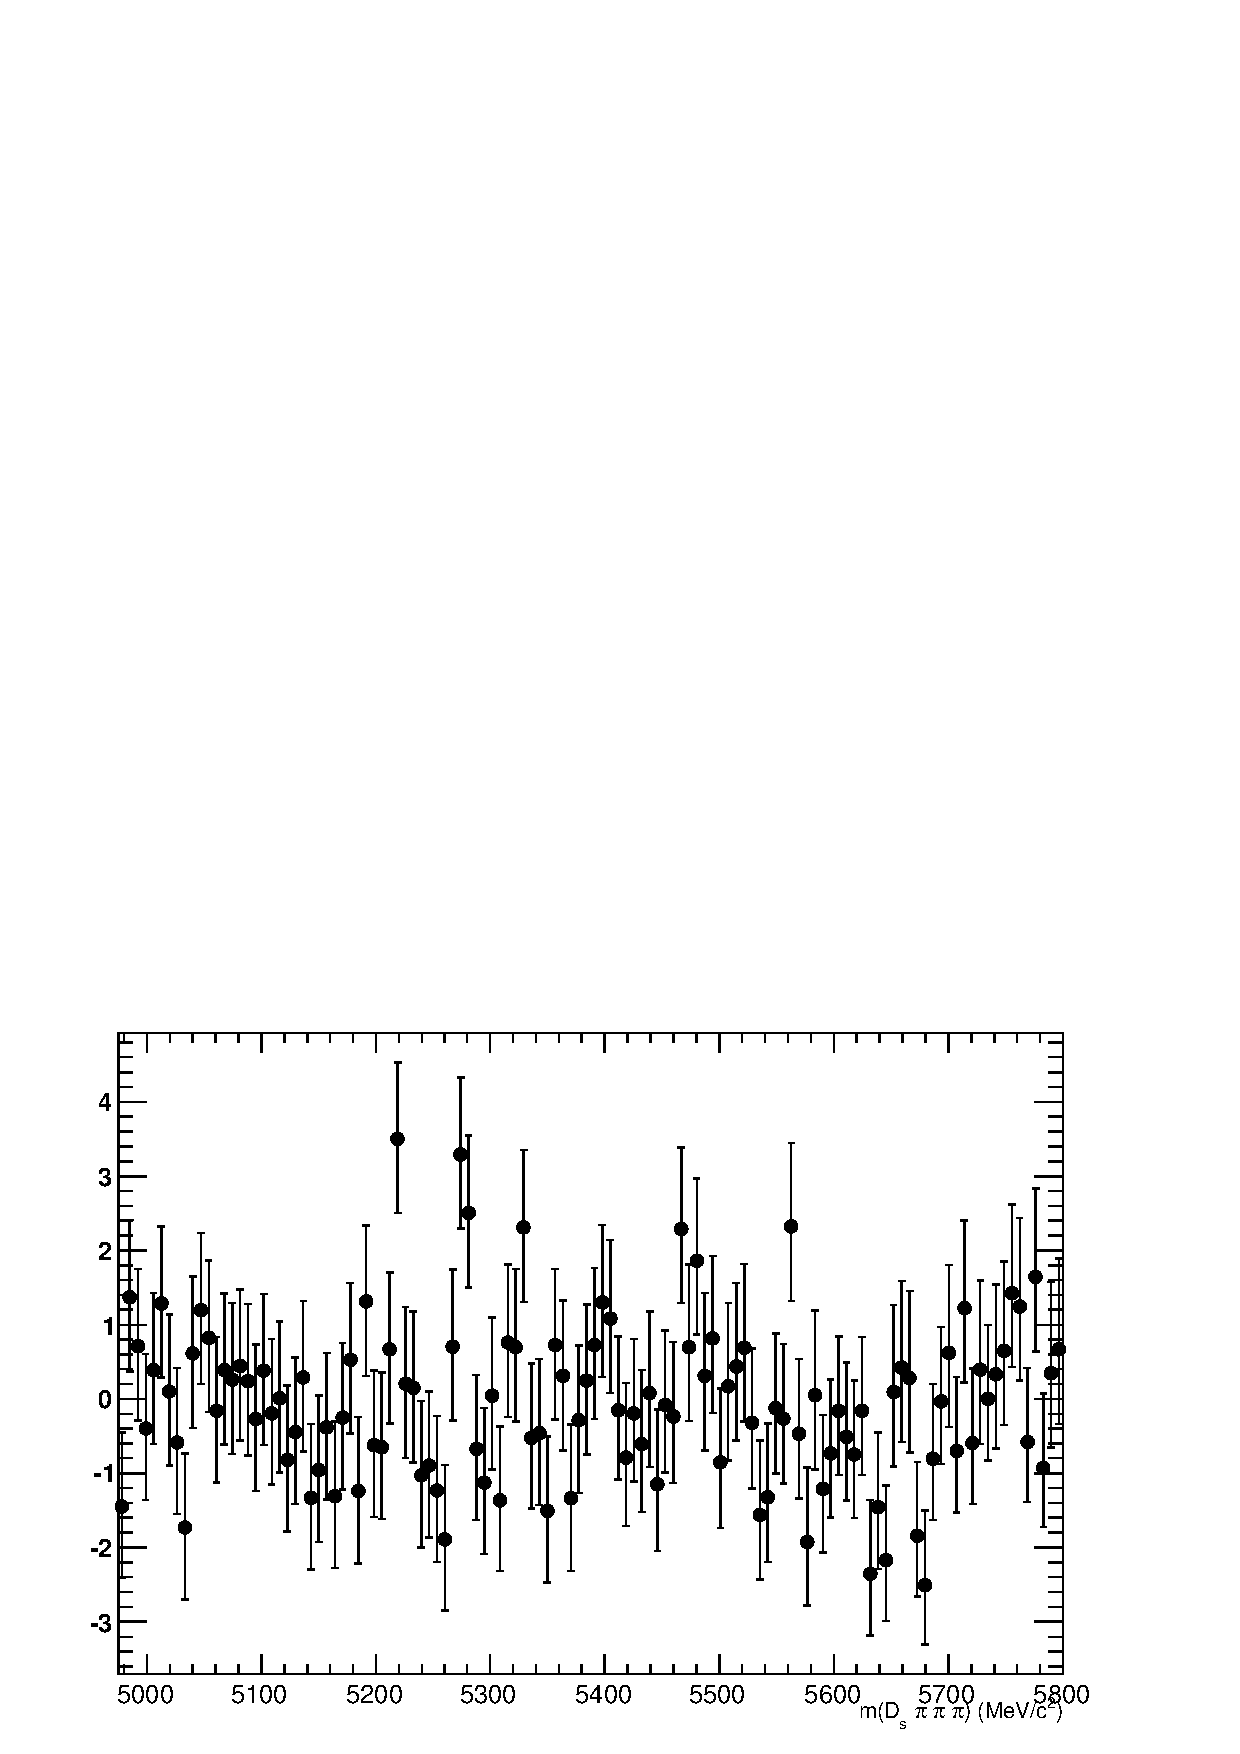
\includegraphics[width=0.49\textwidth,height=1.5cm]{figs/3pi_pull_sim12.pdf}
\caption{Invariant mass distribution of $\Bs\to\Ds\pion\pion\pion$ candidates for (left) 2011 and (right) 2012 data.
The fit described in the text is overlaid. The dashed lines show the (magenta) partially reconstructed and (red) combinatorial component, as well as the (blue) signal component. 
The pull distributions for the simultaneous fit are shown at the lower left and right.}
\label{fig: BsDs3piFit}
\end{figure}

%The determined number of $\Bs\to\Ds\pion\pion\pion$ decays is $8496 \pm 102$ for 2011 data and $19410 \pm 160$ for 2012 data. 
%The determined yield for the partially reconstructed $\Bs\to\Ds^{*}\pion\pion\pion$ background is  (2011) $16904 \pm 299$ and (2012)  $38437 \pm 589$, 
%while the yield for the combinatorial background is (2011) $16066 \pm 304$ and (2012) $35285 \pm 596$.



\subsection{Fit to $\Bs\to\Ds\kaon\pion\pion$ candidates}
\label{subsec: SigFit}

\begin{figure}[h]
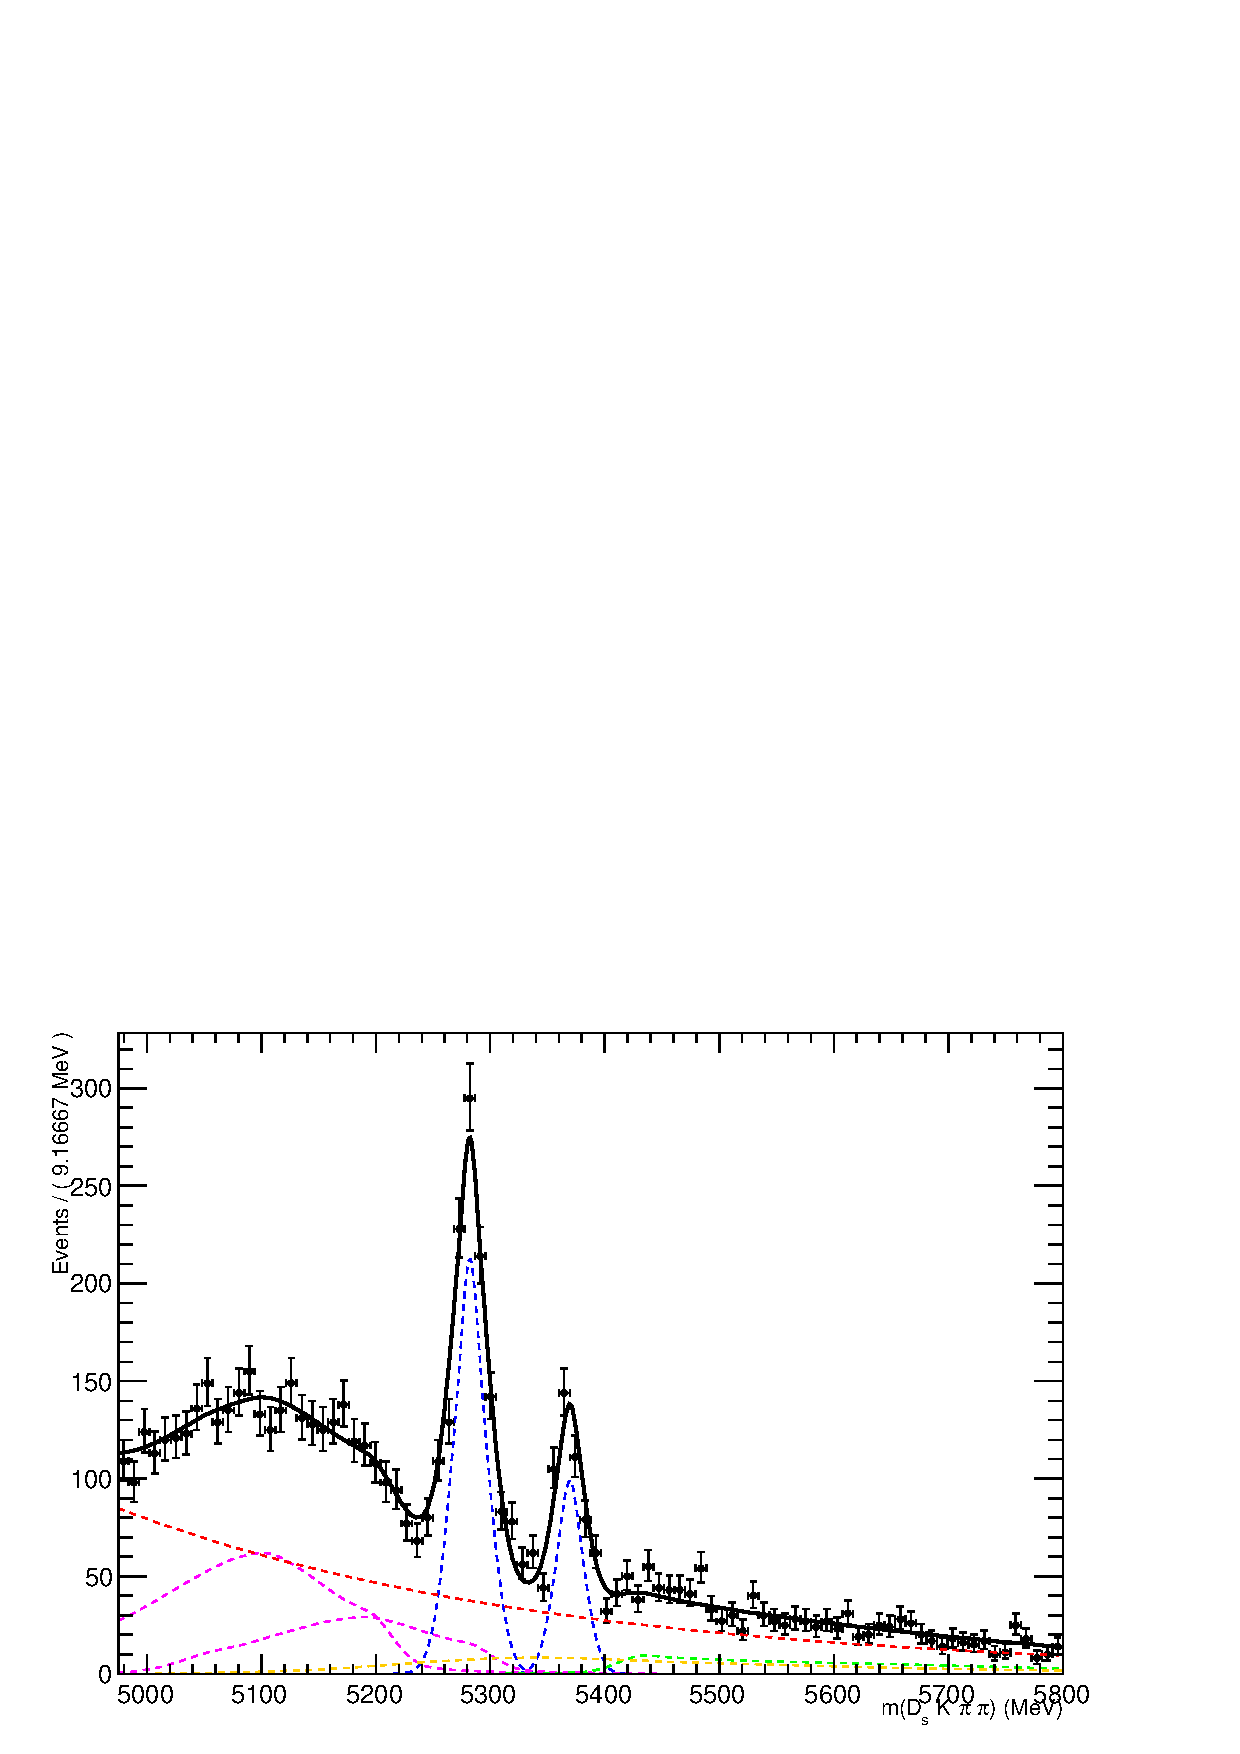
\includegraphics[height=7.cm,width=0.49\textwidth]{figs/BmassFit_sim11.pdf}
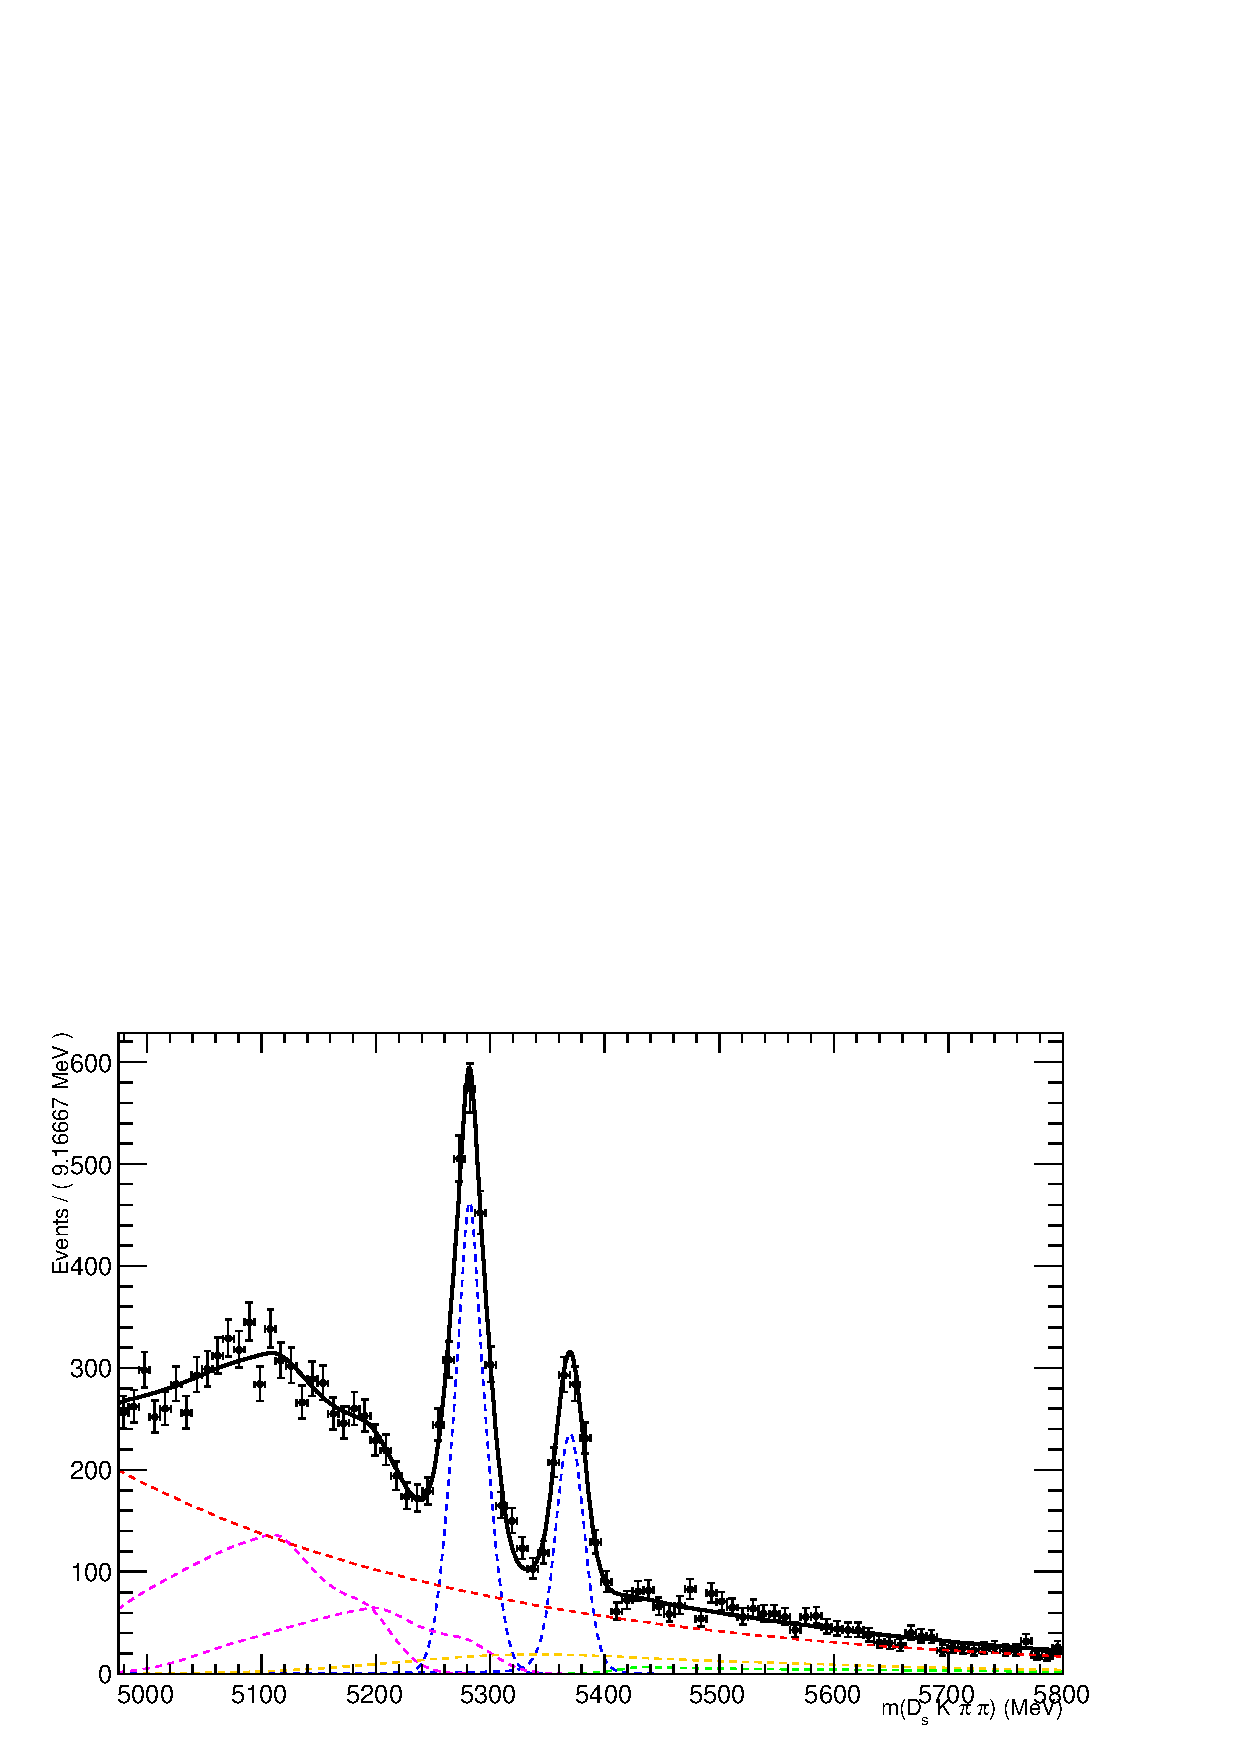
\includegraphics[height=7.cm,width=0.49\textwidth]{figs/BmassFit_sim12.pdf}\\
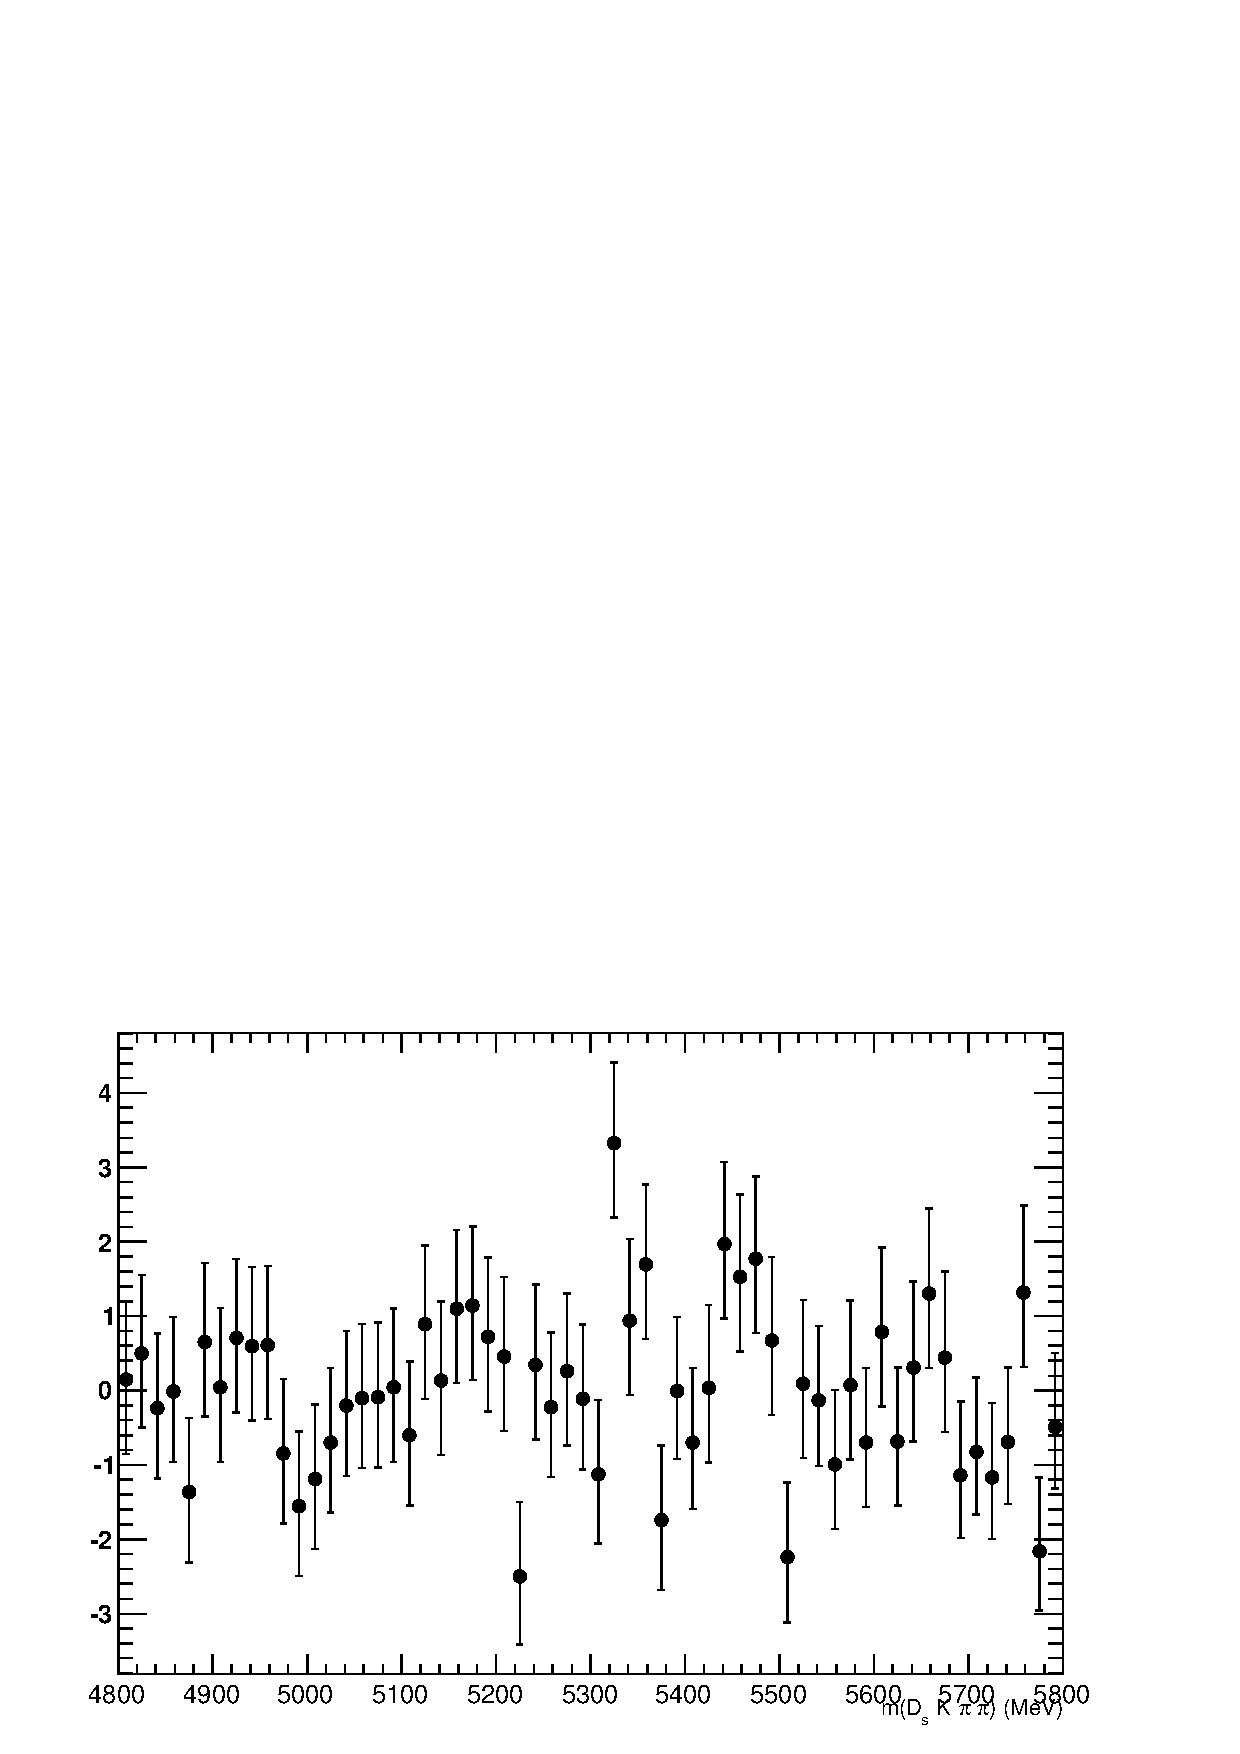
\includegraphics[width=0.49\textwidth,height=1.5cm]{figs/pull_sim11.pdf}
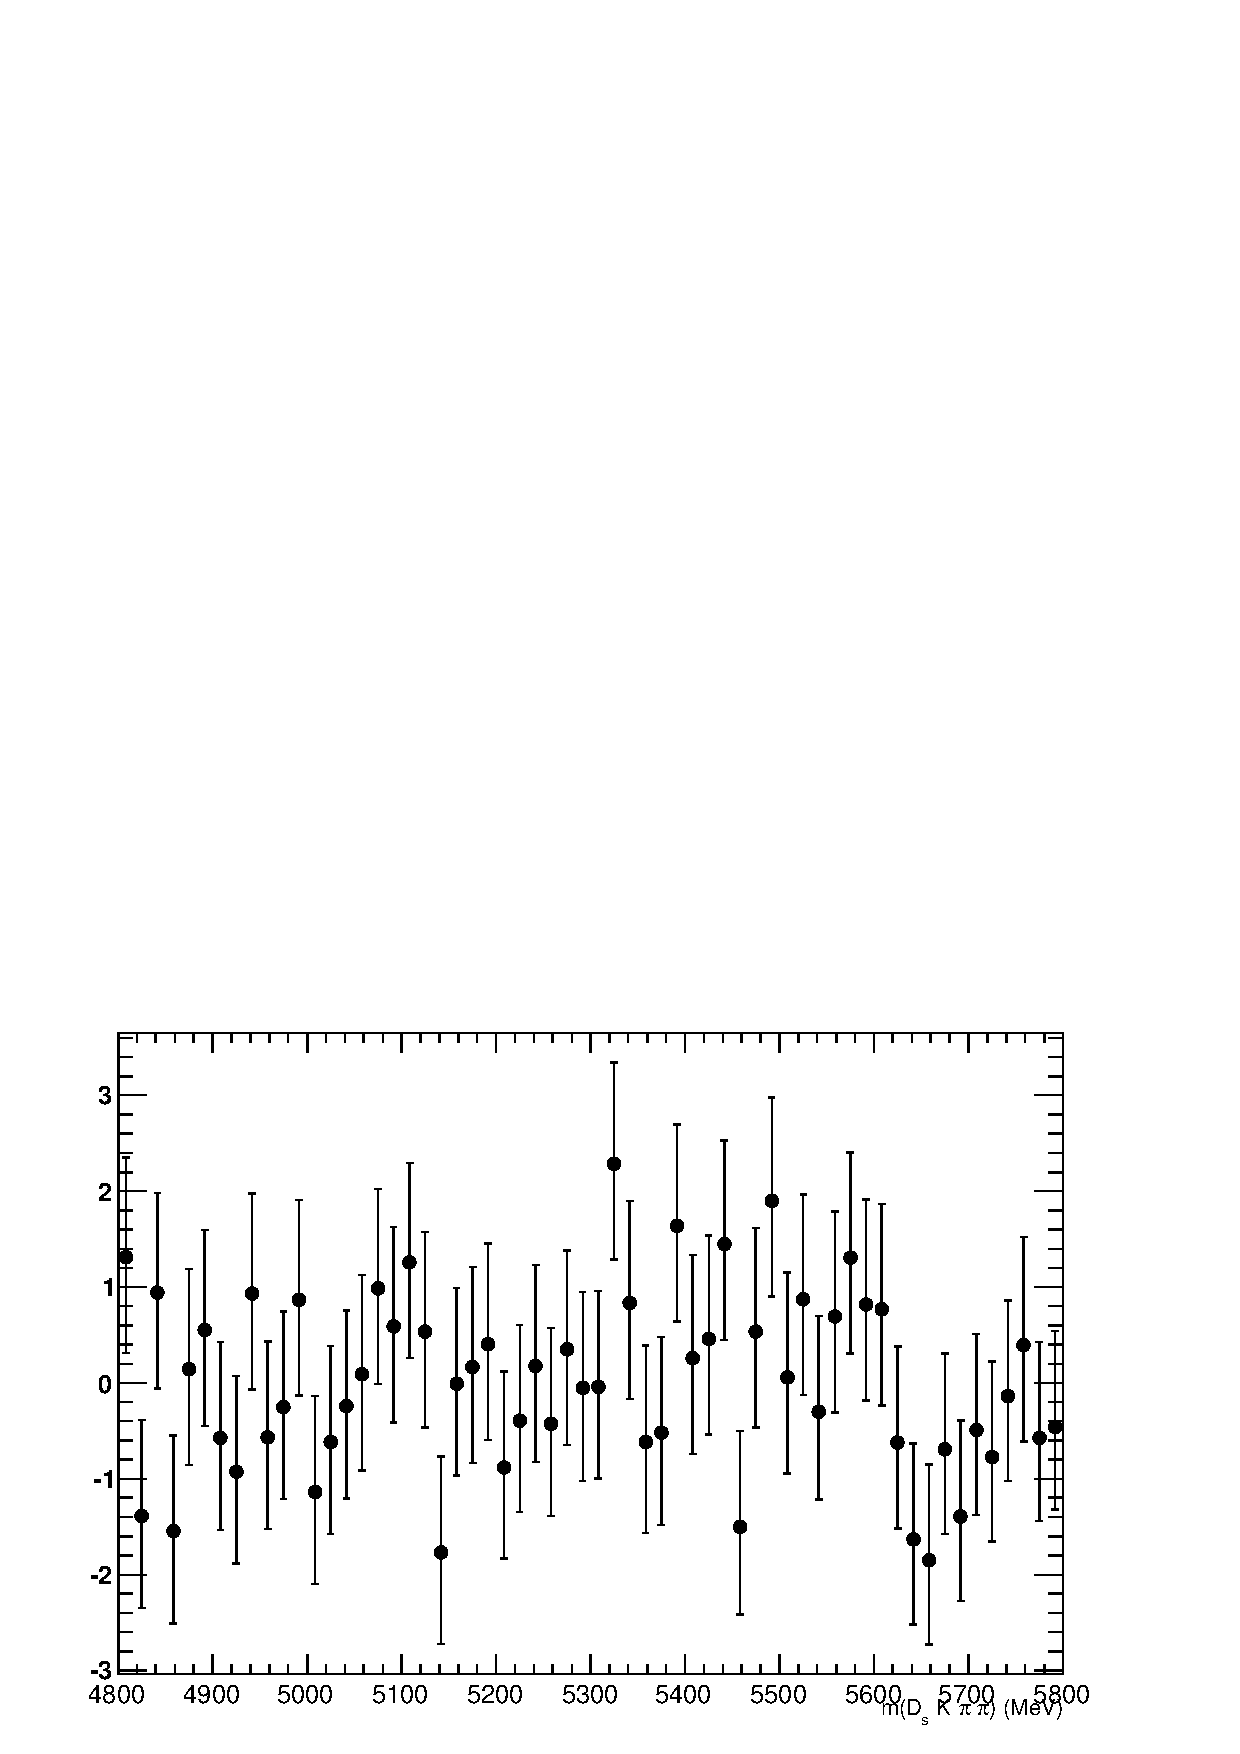
\includegraphics[width=0.49\textwidth,height=1.5cm]{figs/pull_sim12.pdf}
\caption{Invariant mass distribution of $\Bs\to\Ds\kaon\pion\pion$ candidates for (left) 2011 and (right) 2012 data.
A fit described in the text is overlaid. The dashed lines show the (magenta) partially reconstructed and (red) combinatorial background, as well as the (blue) signal component. 
The dashed green line depicts the misID backgrounds and the dashed yellow line depicts the misidentified, partially reconstructed background component. 
The pull distributions for the simultaneous fit are shown at the lower left and right.}
\label{fig: BsDsKpipiFit}
\end{figure}

The shape of the invariant mass distribution of$\Bs\to\Ds\kaon\pion\pion$ candidates is described by the sum of two double Gaussian functions for the $\Bz$ and $\Bs$ signal, 
two sums of three bifurcated Gaussians for the $\Bs$/$\Bz\to\Ds^{*}\kaon\pion\pion$ partially reconstructed background contributions and 
two sums of double Crystal Ball functions for the single misID $\Bs\to\Ds\pion\pion\pion$ and the partially reconstructed, misidentified $\Bs\to\Ds^{*}\pion\pion\pion$ decays. 
A simultaneous unbinned maximum likelihood fit is performed and the result is shown in Fig. \ref{fig: BsDsKpipiFit}.
 

\begin{table}[h]
\centering
\begin{tabular}{l c c}
invariant mass spectrum/fit component & yield 2011 & yield 2012\\
\hline \hline
$m(\Ds\kaon\pion\pion)$    &                  &\\
\hline
$\Bs\to\Ds\kaon\pion\pion$    &  $351 \pm 26$    &  $858 \pm 40$\\
$\Bz\to\Ds\kaon\pion\pion$    &  $821 \pm 41$    &  $1721 \pm 67$\\
$\Bs\to\Ds^{*}\kaon\pion\pion$ &  $629 \pm 68$   &  $1333 \pm 129$\\
$\Bz\to\Ds^{*}\kaon\pion\pion$ &  $1252 \pm 188$ &  $2653 \pm 400$\\
$\Bs\to\Ds\pion\pion\pion$    &  $257$ (fixed)   & $582$ (fixed)\\
$\Bs\to\Ds^{*}\pion\pion\pion$ &  $359$ (fixed)  & $845$ (fixed)\\
combinatorial                 &  $2999 \pm 154$  & $6689 \pm 240$\\
\hline \hline
$m(\Ds\pion\pion\pion)$       &                  &\\
\hline
$\Bs\to\Ds\pion\pion\pion$    &  $7671 \pm 96$  &  $17379 \pm 148$\\
$\Bs\to\Ds^{*}\pion\pion\pion$ & $9984 \pm 193$  & $23479 \pm 357$\\
combinatorial                 & $10341 \pm 204$  & $21737 \pm 373$\\
\hline
\end{tabular}
\caption{Summary of yields from the fits to 2011 and 2012 data.}
\label{tab: SigYields}
\end{table}

